\documentclass[10pt]{article}
\usepackage[utf8]{inputenc}
\usepackage[T1]{fontenc}
\usepackage{amsmath}
\usepackage{amsfonts}
\usepackage{amssymb}
\usepackage[version=4]{mhchem}
\usepackage{stmaryrd}
\usepackage{graphicx}
\usepackage[export]{adjustbox}
\graphicspath{ {./images/} }
\usepackage{bbold}

\begin{document}
Models 14-10-25

$$
I(\lambda) \simeq g\left(x_{0}\right) e^{\lambda f\left(x_{0}\right)} \sqrt{\frac{2 \pi}{\lambda\left(f^{\prime \prime}\left(x_{0}\right)\right)}}
$$

interion max $I(\lambda) \sim \lambda^{-1 / 2} e^{\lambda f\left(x_{0}\right)}$ endpoint (not flot) $\quad I(\lambda) \sim \lambda^{-1} e^{\lambda f\left(x_{0}\right)}$

Lp- norm in real and psis\\
The quontity

$$
\|g\|_{p}:=\left(\int_{a}^{b}|g(t)|^{p} d t\right)^{1 / p} \quad p>0
$$

is colled $p$-norm when the inicynal exists (in Lestegue shase) We want to study the behavior of $\|g\|_{p}$ as $p \rightarrow \infty$. We assume that $g$ has a mique matimum in $t_{0}$ which is an interior point, and $g \in C^{4}(a, b)$.\\
We first study

$$
I(p) \equiv \int_{a}^{b}|g(t)|^{p} d t \quad\|g\|_{p}=I^{1 / p}
$$

and

$$
I=\int_{a}^{b} e^{p \ln |g(t)|} d t
$$

When we applied the Laplace methad we have always assumed that $f$ is continuously chifferentiable. However, if $g$ varishes somewhere in $[a, b]$ then $h / g / \rightarrow-\infty$. However, every neighborherd of points where $g=0$ will gield a negligible contribution to the initgral (i.e. to I for $p \gg 1$ ).

Thus such discontinuities con be neglected. Now we use op. (22)

$$
\begin{aligned}
I(p) & =e^{p \ln \left|g\left(t_{0}\right)\right|} \sqrt{\frac{2 \pi g\left(t_{0}\right)}{p\left|g^{\prime \prime}\left(t_{0}\right)\right|}}\left(1+\partial\left(\frac{1}{p}\right)\right) \\
& =\left|g\left(t_{0}\right)\right|^{p} \sqrt{\frac{2 \pi g\left(t_{0}\right)}{p\left|g^{\prime \prime}\left(t_{0}\right)\right|}}\left(1+\partial\left(\frac{1}{p}\right)\right) \text { as } p \rightarrow \infty
\end{aligned}
$$

Obs: $\quad a>0 \quad \underline{a^{1 / p} p^{-\frac{1}{2 p}}}=e^{\frac{\ln a}{p}} e^{-\frac{\ln p}{2 p}}=$\\
$I^{1 / p}=\left|g\left(t_{0}\right)\right|\left(\frac{2 \pi|g|}{p\left|g^{\prime \prime}\right|}\right)^{\frac{1}{2 p}}+\operatorname{lot}=\left|g\left(t_{0}\right)\right|\left(1-\frac{\ln p}{2 p}+\sigma\left(\frac{1}{p}\right)\right)$\\
hence

$$
\|g\|_{p}=\max _{t \in[a, b]}|g(t)|\left\{1-\frac{\ln p}{2 p}+\cdots\right\} \text { as } p \rightarrow \infty
$$

which gustifies the usual definition

$$
\|g\|_{\infty}=\max _{t \in[a, b]}(g)
$$

Example:\\
Consider the integral

$$
\int_{0}^{\frac{3 \pi}{2}} e^{-\lambda \sin t} f(t) d t \quad \text { as } \quad \lambda \rightarrow \infty
$$

where $f$ is cont. and diff. in $\left[0, \frac{3 \pi}{2}\right]$.\\
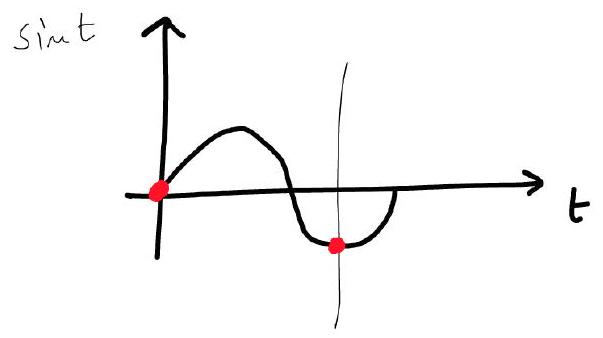
\includegraphics[max width=\textwidth, center]{2025_10_19_11b40f5928aca93f9d20g-3}

We want to consider the contributions from the endpoint mimima $t=0, t=\frac{3 \pi}{2}$. For this we write

$$
I(\lambda)=\underbrace{\int_{0}^{\pi / 2} e^{-\lambda \sin t} f(t) d t}_{I_{1}}+\underbrace{\int_{\pi / 2}^{\lambda \pi / 2} e^{-\lambda \sin t-\lambda} f(t) d t}_{I_{2}}
$$

9.(24) left end point

$$
I_{1}=f(0) \frac{e^{\lambda \cdot 0}}{\lambda \cos (0)}=\frac{f(0)}{\lambda} \text { es } \lambda \rightarrow \infty
$$

el. (23)\\
flat enopoint

$$
I_{2}=f\left(\frac{3 \pi}{2}\right) e^{\lambda \cdot 0} \sqrt{\frac{\pi}{2 \lambda \sin \left(\frac{3 \pi}{2}\right)}} \simeq f\left(\frac{3 \pi}{2}\right) \sqrt{\frac{\pi}{2 \lambda}}
$$

Hence the leading contribution comes from $I_{2}$ and

$$
I(\lambda)=f\left(\frac{3 \pi}{2}\right) e^{\lambda} \sqrt{\frac{\pi}{2 \lambda}}+\text { h.o.t. } \quad \text { as } \quad \lambda \rightarrow 0
$$

The min a $t=0$ is subleadhing and it should be taken into account only at higher order.

Ex: Calculate the leading contribution to

$$
\int_{0}^{\pi} e^{-\lambda \sin t} f(t) d t \quad \text { as } \lambda \rightarrow \infty
$$

\section*{Review of Dynomical Systems}
In mony applications (physics, biology, chemistry...) one has to study nonlinear systems of (antonomons) ODEs:

\[
\left\{\begin{array}{l}
\dot{\vec{x}}(t)=\vec{f}(\vec{x}(t))  \tag{1}\\
\vec{x}(0)=\vec{x}_{0}
\end{array}\right.
\]

where $\vec{x}(t)=\left(x_{1}(t), \ldots, x_{N}(t)\right) \in U \subseteq \mathbb{R}^{N}, U$ is some open commected set of reals.\\
With any $\vec{x}$ we associate a vector $\vec{f}$, the set of these vectors is called vector field. The domain $U$, where $\vec{f}$ is supposed to be continuous and differentiable, is colled the phose space.\\
The solutions $\vec{x}\left(t, x_{0}\right)$ of the system (1) describe smooth aurves a $t$ chonges: they are called trajectories which are porometric curves in the phose space.

\section*{Example:}
Let's consider $(N=1)$

$$
\dot{x}(t)=\sin [x(t)]
$$

$\partial_{n}$ this case the vector field is 1-chim. and coincides with the $x$-axis.\\
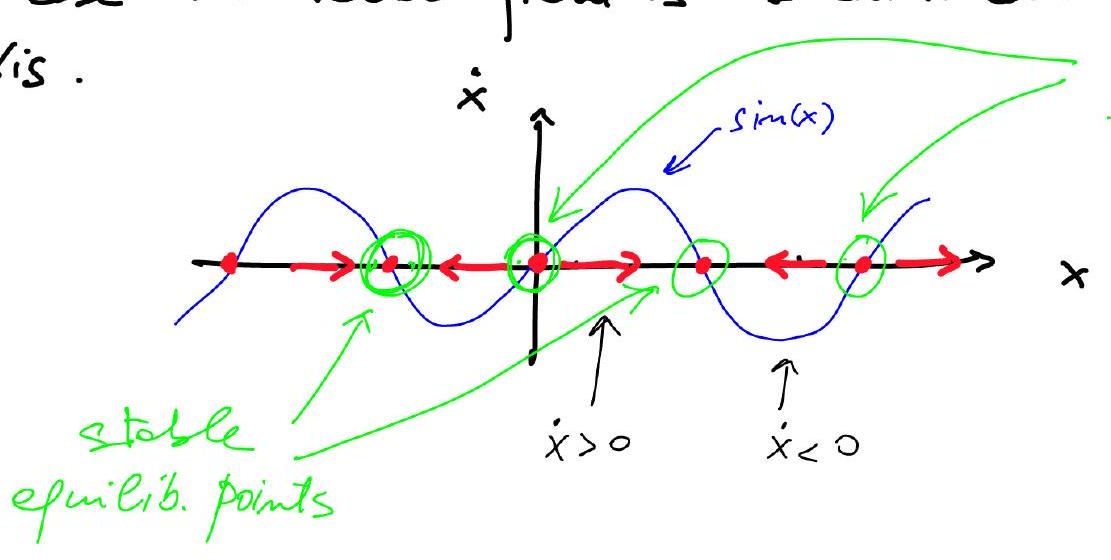
\includegraphics[max width=\textwidth]{2025_10_19_11b40f5928aca93f9d20g-4} equil. points

In the $N=2$ cose

$$
\left\{\begin{array}{l}
\dot{x}=1 \\
\dot{y}=x^{2}+y^{2}
\end{array}\right.
$$

the vector field is 2 dim. and we have a map

$$
\vec{x}=(x, y) \longrightarrow \vec{f}(\vec{x})=\left(1, x^{2}+y^{2}\right)
$$

\begin{center}
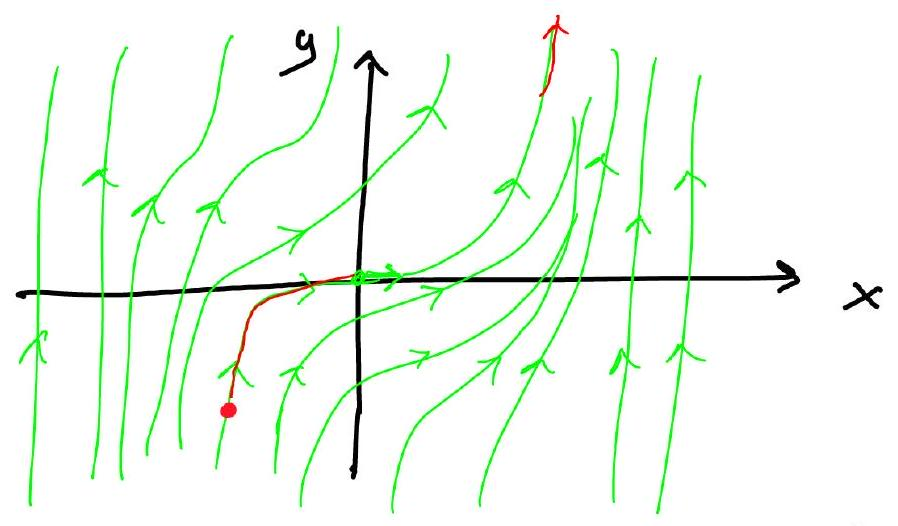
\includegraphics[max width=\textwidth]{2025_10_19_11b40f5928aca93f9d20g-5}
\end{center}

$$
\begin{array}{ll}
\hat{x} & \hat{y} \\
\dot{y}
\end{array}
$$

$$
(0,0) \longrightarrow(1,0)
$$

In general the vector field $\vec{f}$ is tengent to a trajectory in every point. In fact, let $\vec{x}(t)$ be a trajectory, then the ep. of a tengent line to the trajectory at a point $\vec{x}_{a} \equiv \vec{x}\left(t_{a}\right)$ is

$$
\vec{Y}(u)=\vec{x}_{a}+\left(u-t_{a}\right) \dot{\vec{x}}\left(t_{a}\right)=\vec{x}_{a}+\left(u-t_{a}\right) \vec{f}\left(\vec{x}_{a}\right)
$$

thus $\vec{f}$ is the directional vector of the straight line $\vec{Y}(a)$.\\
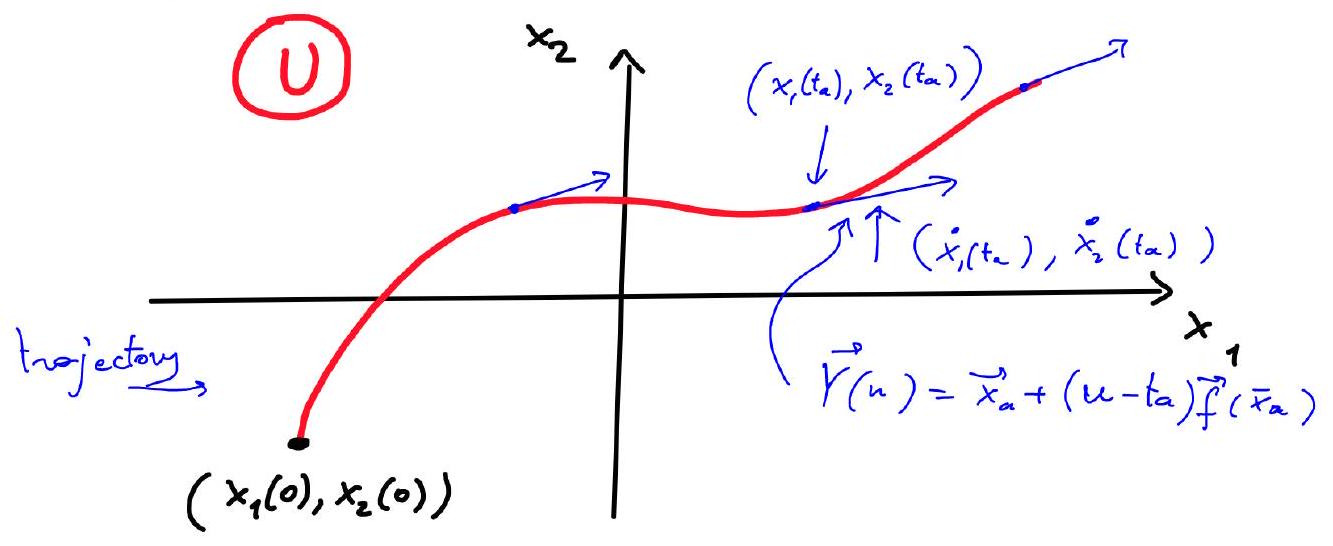
\includegraphics[max width=\textwidth, center]{2025_10_19_11b40f5928aca93f9d20g-5(1)}


\begin{gather*}
N=2 \\
\left\{\begin{array}{l}
\dot{x}_{1}=f_{2}\left(x_{1}, x_{2}\right) \\
\dot{x}_{2}=f_{2}\left(x_{1}, x_{2}\right)
\end{array}\right.  \tag{2}\\
\text { (2) }
\end{gather*}


By flowing along the vector field, a point traces out the trajectory $\vec{x}(t)$, a curve in the phase space $U$ or a sol. of (2).

A phose partzait is a set of trajectories with the indication of the directions of the vector field.\\
As we commot sobre the system (1) in general, we would like to know at least some properties.\\
Sometimes it is useful to study nullclines, defined es subspeces (or monifolds) where $\dot{x}_{i}=0$ for a give i. $\mathcal{H} N=2$ we may get simple curves

$$
\begin{array}{r}
\dot{x}_{1}=0 \Rightarrow f_{1}\left(x_{1}, x_{2}\right)=0 \Rightarrow \\
\text { persibly } \\
x_{2}^{(1)}=g^{(1)}\left(x_{1}\right) \\
x_{2}^{(2)}=g^{(2)}\left(x_{1}\right)
\end{array}
$$

Twe interesting examples

\begin{enumerate}
  \item Find a solution of $\dot{y}=y^{2}$ with i.c. $y(0)=1$.
\end{enumerate}

Con we then find $y(2)$ ?\\
From $\int \frac{d y}{y^{2}}=t-c, y=\frac{1}{c-t}, y(0)=1 \Rightarrow c=1$

$$
y(t)=\frac{1}{1-t} \quad \rightarrow y(2)=-1
$$

As $\dot{y}(t) \geqslant 0, y$ is an increasing function of time but $y(2)=-1$ ! Actually, the solution exists only in the interval $(0,1)$ as it blows up a $t=1$.\\
Solutions may exist only within finite intervals of time or the may not exist for some initial conditions or may not exist at all.\\
2) Find a solution of $j=\sqrt{y}$ for which $y(0)=0$. Find $y(2)$.

$$
\int \frac{d y}{\sqrt{y}}=2 \sqrt{y}=t-c, \quad y=\frac{(t-c)^{2}}{4} \text { but } y(0)=0, y(t)=\frac{t^{2}}{4}
$$

hence $y(2)=1$. But!

However $y(t)=0$ satisfies the of, and the imit. cond. Even wase:

$$
y(t)=\left\{\begin{array}{cc}
0 \quad 0 \leq t \leq T & T \text { is anbitary } \\
\frac{(t-T)^{2}}{4} \quad t>T & T>0 .
\end{array}\right.
$$

is a solution with the same imitial constition! So there are infinitely mony solutions, so asking $y(2)$ is meomingles.\\
Sol. to init. val problems may not be unique.

\section*{Picard's theorem}
If $\vec{f}$ is continuous and $\frac{\partial f_{i}}{\partial x_{j}}$ are also continuous for all indexes $i j j$ in $U$, then for any $\vec{x}_{0} \in U$ the initial value problem difined in (1) admits a solution on some interval $t \in[-\delta, \delta], \delta>0$, and this salution is unique.

Obs: in this cese trajectories do not intersect.

\section*{Fixed points}
The fixed points of $\varphi$. (4) are the simplest to study as time is not relevant. Indeed, fixed points are the zeros of $\vec{f}$ : namely, $\vec{x}^{*}$ is a fixed point if


\begin{equation*}
\vec{f}\left(\vec{x}^{*}\right)=\overrightarrow{0} \tag{3}
\end{equation*}


Worning: even thoyh an $O D E$ has some fixed points, that does not imply that the dymamics (the imit. Val. solut.) seach them!


\end{document}